%%%%%%%%%%%%%
%  Ch1 : Generalities  %
%%%%%%%%%%%%%

\chapter{Generalities}
\section{Fundamental laws}
\subsubsection{Reminder}
	Let's first remind the 3 basic principles of \textit{Fluid mechanics I} : \\
	
	\begin{itemize}
		\item[•] \textbf{Mass conservation :} \textit{The mass of a closed system remains constant in time.}\\
		This is much a definition of a closed system than a principle. We have to notice that related to Einstein law of relativity, $E = mc^2$, mass must vary with energy. But if we exclude nuclear reactions, our approximation is valid. Indeed, the square of light velocity has a greater impact on energy than the mass term. If the energy exchange is huge like in nuclear reaction, mass vary, but in smaller energies domain (combustion for example), the mass can be considered as constant. \\
		
		\item[•] \textbf{Newton's law :} \textit{the time rate of change of momentum of a closed system is equal to the sum of the forces applied on the system.} \\
		
		\item[•] \textbf{First principle of thermodynamics :} \textit{the time rate of change of the total energy of a closed system is equal to the sum of the power of the forces applied on the system and the thermal power provided to the system.}
	\end{itemize}		
	
	\subsubsection{Useful equations}
	
	\begin{wrapfigure}[9]{l}{4cm}
	\vspace{-5mm}
	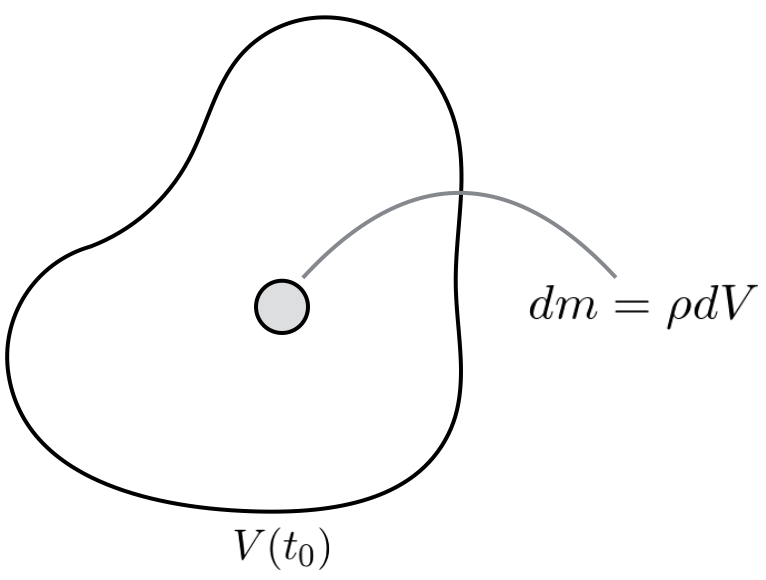
\includegraphics[scale=0.3]{ch1/1}
	\captionof{figure}{}
	\label{fig:1.1}
	\end{wrapfigure}
	Let's consider the integral on a moving volume of a function depending on time and position $f(\vec{x},t)$. Imagine that \autoref{fig:1.1} represents the moving volume at initial time containing mass $m$. An infinitesimal part of that volume contains an infinitesimal mass $dm = \rho dV$, where $\rho$ is mass density. We deduce the expression of the total mass at any time by that of the initial time  
	\begin{equation}
		M(t_0) = \int _{V(t_0)}\rho (\vec{x},t_0)\, dV \qquad \Rightarrow M(t) = \int _{V(t)}\rho (\vec{x},t)\, dV
	\end{equation}
	By considering $\rho (\vec{x},t)$ as $f(\vec{x},t)$, the derivative of the integral is given by
	
	\begin{center}
	\theor{\textbf{Reynolds transport theorem}
	\begin{equation}
		\frac{d}{dt}\int _{V(t)}f (\vec{x},t)\, dV = \int _{V(t)} \frac{\D f}{\D t} (\vec{x},t)\, dV + \oint _{S(t) = \D V(t)} f(\vec{x},t) \vec{b}\, \vec{n}\, dS
	\end{equation}
	where $\vec{b}$ is the surface displacement velocity. }
	\end{center}
	
	The second equation that will be used in the developement is given by
	\begin{center}
	\theor{\textbf{Gauss theorem}
	\begin{equation}
		\oint _{S = \D V} \vec{a} \, \vec{n} \, dS = \int _V \nabla \vec{a}\, dV
	\end{equation}}
	\end{center}
	
	\subsection{Mass conservation equation}
	If $V(t)$ is the moving volume occupied by the closed system as time varies, then by definition of a closed system $\frac{dM(t)}{dt} = 0$. The corresponding equation using Reynolds transport theorem is 
	\begin{equation}
		M(t) = \int _{V(t)} \rho\, dV \qquad \Rightarrow \frac{dM(t)}{dt} = \int _{V(t)} \frac{\D \rho}{\D t}\, dV + \oint _{S(t) = \D V(t)} \rho\, \vec{b}\, \vec{n}\, dS = 0
	\end{equation}
	\begin{wrapfigure}[9]{l}{3cm}
	\vspace{-5mm}
	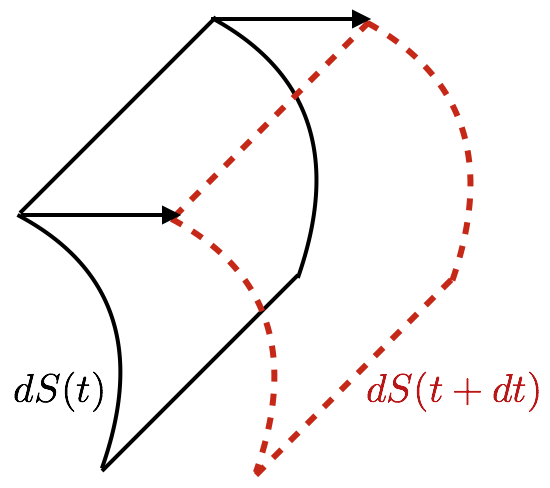
\includegraphics[scale=0.3]{ch1/2}
	\captionof{figure}{}
	\label{fig:1.2}
	\end{wrapfigure}
	We have to express that this volume is not traversed by material. There is no flux of fluid and the particles in the volume are always the same. By definition, the infinitesimal distance traveled by the surface and the fluid are
	\begin{equation}
		d\vec{x} = \vec{b}\, dt \qquad and \qquad d\vec{x}' = \vec{u}\, dt
	\end{equation}	 
	where $\vec{u}$ is the fluid velocity. Under wich condition do we know that the fluid has not traversed the boundary ? We have to define the relative dispolacement $d\vec{x}'-d\vec{x}$ of the fluid in regard to the fluid. For a closed system 
	\begin{equation}
	\begin{aligned}
		(d\vec{x}'-d\vec{x})\cdot \vec{n} = 0 \quad &\Leftrightarrow \quad dt (\vec{u}-\vec{b})\cdot \vec{n} = 0 \quad \Leftrightarrow \quad (\vec{u}-\vec{b})\cdot \vec{n} = 0 \\
		&\Rightarrow \quad \vec{b} \vec{n} = \vec{u} \vec{n}
		\end{aligned}
	\end{equation}
	\begin{center}
	\theor{\textbf{Mass conservation equation for closed systems (integral form)}
	\begin{equation}
		\int _{V(t)} \frac{\D \rho}{\D t}\, dV + \oint _{S(t) = \D V(t)} \rho\, \underbrace{\vec{b}\, \vec{n}}_{=\vec{u}\, \vec{n}}\, dS =0
		\label{eq:1.7}
	\end{equation}}
	\end{center}
	
	How to write this equation in a different way ? Let's consider now a fixed open system composed of fluid particles in the fixed volume $V_0(t) = V(t_0)$. Similarly to the previous point, the mass variation in this fixed volume is expressed like 
	\begin{equation}
		M_0(t) = \int _{V_0(t)} \rho\, dV \qquad 
		\Rightarrow \int _{V_0(t)} \frac{\D \rho}{\D t}\, dV + \oint _{S_0(t) = \D V_0(t)} \rho\, \vec{b}\, \vec{n}\, dS.
	\end{equation}
	The volume integral expresses the variable mass in the fixed volume and the surface integral is nul due to the nul surface velocity (since the volume is fixed). This relation enables us to write the 
	\begin{center}
	\theor{\textbf{Mass conservation equation for fixed open systems (integral form)}
	\begin{equation}
		\frac{dM_0}{dt} + \underbrace{\oint _{S_0(t) = \D V_0(t)} \rho\, \vec{u}\, \vec{n}\, dS = 0}_{\mbox{mass flow out of the system}}
	\end{equation}}
	\end{center}	
	Let's finally consider an arbitrary open system containing fluid particles in a moving volume $V_*(t)$ such that $V_*(t_0) = V(t_0) = V_0$. Similarly we have using the Reynolds transport theorem
	\begin{equation}
		M_*(t) = \int _{V_*(t)} \rho\, dV \qquad \Rightarrow \frac{dM_*(t)}{dt} = \int _{V_*(t)} \frac{\D \rho}{\D t}\, dV + \oint _{S_*(t) = \D V_*(t)} \rho\, \vec{b}\, \vec{n}\, dS
	\end{equation}
	Using the definition of the volume at $t=t_0$, we can equalize the volume integral with that of \autoref{eq:1.7} to find 
	\begin{center}
	\theor{\textbf{Mass conservation equation for arbitrary open systems (integral form)}
	\begin{equation}
		\frac{dM_*(t_0)}{dt} + \oint _{S(t_0) = \D V(t_0)} \rho (\vec{u}-\vec{b})\, \vec{n}\, dS = 0
	\end{equation}}
	\end{center}	
	
	Let's now take \autoref{eq:1.7} again and apply Gauss theorem
	\begin{equation}
	\begin{aligned}
		\int _{V(t)} \frac{\D \rho}{\D t}\, dV + \oint _{S(t) = \D V(t)} \rho \underbrace{\vec{u}\, \vec{n}}_{\vec{a}}\, &dS =0 \qquad with \qquad 
		\oint _{S(t)} \rho\, \underbrace{\vec{u}\, \vec{n}}_{\vec{a}}\, dS = \int _{V(t)} \nabla \rho \vec{u} \, dV \\
		&\Leftrightarrow \int _{V(t)} \left[ \frac{\D \rho}{\D t} + \nabla \rho \vec{u} \right] \,dV
		\end{aligned}
	\end{equation}
	For this last equation to be true for all systems, the integrated term must be equal to zero 
	\begin{center}
	\theor{\textbf{Mass conservation equation (differential form (1) - divergent form)}
	\begin{equation}
		\frac{\D \rho}{\D t} + \nabla \rho \vec{u} = 0
		\label{eq:1.13}
	\end{equation}}
	\end{center}
	
	\begin{wrapfigure}[4]{l}{4cm}
	\vspace{-5mm}
	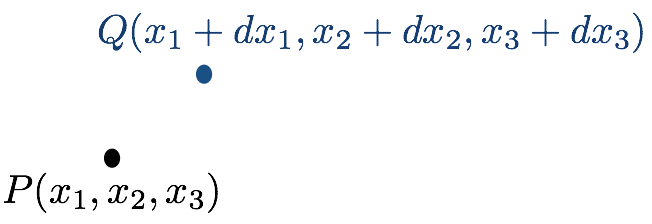
\includegraphics[scale=0.35]{ch1/3}
	\captionof{figure}{}
	\label{fig:1.3}
	\end{wrapfigure}
	In order to find the second differential form, let's consider 2 points Q and P as described in \autoref{fig:1.3}. The difference of density between the 2 points is \\\\\\
	\begin{equation}
	\begin{aligned}
		\rho _Q(t+dt) - \rho _P(t) &= \rho (x_1+dx_1,x_2+dx_2,x_3+dx_3,t+dt) - \rho (x_1,x_2,x_3)  \\
		&= d\rho = \frac{\D \rho}{\D x_1}dx_1 + \frac{\D \rho}{\D x_2}dx_2 + \frac{\D \rho}{\D x_3}dx_3 + \frac{\D \rho}{\D t}dt
		\end{aligned}
		\label{eq:1.14}
	\end{equation}
	In general, the fluid particles at $P(t)$ and $Q(t+dt)$ are different. However, if $dx_1 = u_1 dt, dx_2 = u_2 dt, dx_3 = u_3 dt$, then the fluid particles at the 2 points are the same. By making appear these velocities in \autoref{eq:1.14}, 
	\begin{equation}
		d\rho = \left( \frac{\D \rho}{\D x_1}u_1 + \frac{\D \rho}{\D x_2}u_2 + \frac{\D \rho}{\D x_3}u_3 + \frac{\D \rho}{\D t}\right) dt
	\end{equation}
	Finally, after dividing by $dt$ the 2 members of the equation, we obtain the definition of the time rate of change of density when I follow the fluid $\dot{\rho}$. As \autoref{eq:1.13} can be expressed in term of indicial notation like 
	\begin{equation}
		\frac{\D \rho}{\D t} + u_i \frac{\D\rho}{\D x_i} + \rho \frac{\D u_i}{\D x_i} = 0 
	\end{equation}
	Replacing the sum of first and second term by $\dot{\rho}$ gives the last form
	\begin{center}
	\theor{
	\textbf{Mass conservation equation (differential form (2) - substancial form)}
	\begin{equation}
	\dot{\rho} + \rho \nabla \vec{u} = 0
	\end{equation}
	}
	\end{center}
	
	\subsection{Newton's second law : Momentum equation}
	Momentum in that course is noted $\vec{P}(t)$. 
	